\documentclass[12pt]{article}
\usepackage[utf8]{inputenc}
\usepackage{float}
\usepackage{amsmath}


\usepackage[hmargin=3cm,vmargin=6.0cm]{geometry}
%\topmargin=0cm
\topmargin=-2cm
\addtolength{\textheight}{6.5cm}
\addtolength{\textwidth}{2.0cm}
%\setlength{\leftmargin}{-5cm}
\setlength{\oddsidemargin}{0.0cm}
\setlength{\evensidemargin}{0.0cm}

%misc libraries goes here
\usepackage{tikz}


\begin{document}

\section*{Student Information } 
%Write your full name and id number between the colon and newline
%Put one empty space character after colon and before newline
Full Name : Emre Berk Kaya \\
Id Number : 2380590 \\

% Write your answers below the section tags
\section*{Answer 1}
\subsection*{a)}
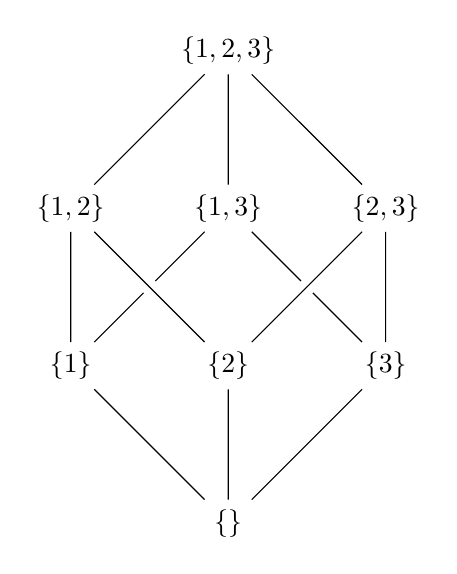
\begin{tikzpicture}
  \node (max) at (0,4) {$\{1,2,3\}$};
  \node (a) at (-2,2) {$\{1,2\}$};
  \node (b) at (0,2) {$\{1,3\}$};
  \node (c) at (2,2) {$\{2,3\}$};
  \node (d) at (-2,0) {$\{1\}$};
  \node (e) at (0,0) {$\{2\}$};
  \node (f) at (2,0) {$\{3\}$};
  \node (min) at (0,-2) {$\{\}$};
  \draw (min) -- (d) -- (a) -- (max) -- (b) -- (f)
  (e) -- (min) -- (f) -- (c) -- (max)
  (d) -- (b);
  \draw[preaction={draw=white, -,line width=6pt}] (a) -- (e) -- (c);
\end{tikzpicture}
\paragraph*{b)}
Since all subsets of the set $\{1,2,3\}$ have both greates lower bound and least upper bound, it is a lattice.

\paragraph*{c)}
For every subset $s$ in $A$, $s \subseteq \{1,2,3\}$. The maximal element is $\{1,2,3\}$.

\paragraph*{d)}
For every subset $s$ in $A$, $\{\} \subseteq s$. The minimal element is $\{\}$.

\paragraph*{e)}
$\{1,2,3\}$ is the upper element in the Hasse diagram, it is the greatest element.

\paragraph*{f)}
$\{\}$ is the bottom element in the Hasse diagram, it is the least element.

\paragraph*{g)}
$\{1,3\}$ is the least upper bound for $\{1\}$ and $\{3\}$.


\newpage


\section*{Answer 2}
\paragraph{a)}
14
\paragraph{b)}
14
\paragraph*{c)}
14
\subsection*{d)}
\begin{figure}[H]
	\centering
	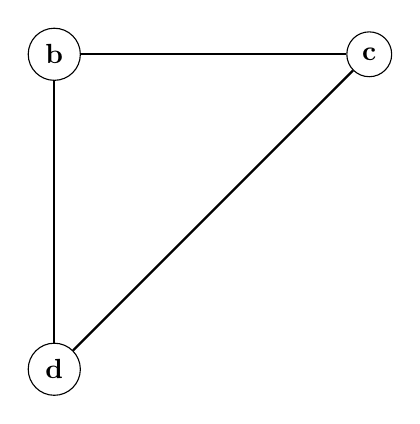
\begin{tikzpicture}
	
	\node[shape=circle,draw=black] (b) at (0, 4)     {\textbf{b}};
	\node[shape=circle,draw=black] (c) at (4, 4)     {\textbf{c}};
	%\node[shape=circle,draw=black] (c) at (6, 2)     {\textbf{c}};
	%\node[shape=circle,draw=black] (d) at (4, 0)     {\textbf{d}};
	\node[shape=circle,draw=black] (d) at (0, 0)     {\textbf{d}};
	
	
	\path[-, thick] (b) edge (c);
	\path[-, thick] (b) edge (d);
	\path[-, thick] (d) edge (c);
	
	\end{tikzpicture} 
	
	\caption{The underlying complete graph of G.}	
	\label{fig:t2}
\end{figure}

\paragraph*{e)} It is not a bipartite graph. If the edges between $a-e$ and $b-d$ removed, it will be a bipartite graph.

\paragraph*{f)} We can select two directions for each edge. The number of directed graphs is $2^7$.

\paragraph*{g)} One example of simple longest path is $a-e-d-b-c$ and the length is 4.

\paragraph*{h)} Since it is a connected graph, every node have a connection with each other. Number of connected components is 1.

\paragraph*{i)} Since all components do not have even degree, there is no Euler circuit.

\paragraph*{j)} $d-c-b-a-e-b-d-e$ is an Euler path.

\paragraph*{k)} $a-b-c-d-e-a$ is an example of Hamilton circuit.

\paragraph*{l)} $a-e-d-b-c$ is an example of Hamilton path.


\section*{Answer 3}

We can complete the mapping as follows: \\
\begin{itemize}
\begin{minipage}{0.4\linewidth}
    \item a to a'
    \item b to c'
    \item c to e'
    \item d to g'
    \end{minipage}
    \begin{minipage}{0.4\linewidth}
    \item e to b'
    \item f to h'
    \item g to d'
    \item h to f'
    \end{minipage}
\end{itemize}
Thus, they are isomorphic.

\section*{Answer 4}

\begin{center}
\begin{tabular}{ c c c c c c c c c c c c c }
 $ $ & current & a & b & c & d & e & f & g & h & i & j & k \\
 step 1 & a & 0 & $3$ & $\infty$ & $\infty$ & $5$ & $\infty$ & $\infty$ & $4$ & $\infty$ & $\infty$ & $\infty$ \\ 
 step 2 & b & 0 & $3$ & $5$ & $\infty$ & $5$ & $10$ & $\infty$ & $4$ & $\infty$ & $\infty$ & $\infty$ \\ 
 step 3 & h & 0 & $3$ & $5$ & $\infty$ & $5$ & $9$ & $\infty$ & $4$ & $6$ & $\infty$ & $\infty$ \\ 
 step 4 & c & 0 & $3$ & $5$ & $8$ & $5$ & $7$ & $11$ & $4$ & $6$ & $\infty$ & $\infty$ \\ 
 step 5 & e & 0 & $3$ & $5$ & $8$ & $5$ & $7$ & $11$ & $4$ & $6$ & $\infty$ & $\infty$ \\ 
 step 6 & i & 0 & $3$ & $5$ & $8$ & $5$ & $7$ & $11$ & $4$ & $6$ & $12$ & $\infty$ \\ 
 step 7 & f & 0 & $3$ & $5$ & $8$ & $5$ & $7$ & $11$ & $4$ & $6$ & $10$ & $\infty$ \\ 
 step 7 & d & 0 & $3$ & $5$ & $8$ & $5$ & $7$ & $11$ & $4$ & $6$ & $10$ & $10$ \\ 
 step 8 & j & stop \\ 
\end{tabular}
\end{center}
The shortest path is $a-b-c-f-j$.

\section*{Answer 5}
\subsection*{a)}
Finding minimum spanning tree with Prim's Algorithm:
We are choosing the edge not forming a cycle with smallest weight and in the neighborhood of current tree in each step.
\begin{itemize}
\item Take $a-b$.
\item Take $a-d$.
\item Take $b-c$.
\item $c-e$ and $c-f$ have the same weight. We can take one of them. Take $c-f$.
\item Take $f-e$. 
\item From this point, we can not go to an edge who does not form a cycle. Then we found the minimum spanning tree.
\end{itemize}
\subsection*{b)}
\begin{figure}[H]
	\centering
	\begin{tikzpicture}
	
	\node[shape=circle,draw=black] (b) at (7, 7.5)     {\textbf{b}};
	\node[shape=circle,draw=black] (a) at (3, 7.5)     {\textbf{a}};
	\node[shape=circle,draw=black] (c) at (11, 7.5)     {\textbf{c}};
	\node[shape=circle,draw=black] (d) at (3, 5)     {\textbf{d}};
	\node[shape=circle,draw=black] (f) at (11, 5)     {\textbf{f}};
	\node[shape=circle,draw=black] (e) at (7, 5)    {\textbf{e}};
	
	\path[-] (f) edge (e);
	\path[-] (c) edge (f);
	\path[-] (b) edge (c);
	\path[-] (b) edge (a);
	\path[-] (a) edge (d);
	
	\end{tikzpicture} 
	\caption{Minimum Spanning Tree in Question 5.}	
	\label{fig:t5}
\end{figure}

\subsection*{c)} 
It is not unique. For example, we could choose $c-e$ instead of $c-f$ in the algorithm. This results in different tree.
  
\section*{Answer 6}
\paragraph*{a)} There are 13 vertices, 12 edges in $T$. The height is 4.

\paragraph*{b)} w-s-m-t-q-x-n-y-u-z-v-r-p

\paragraph*{c)} s-w-q-m-t-p-x-u-n-y-r-v-z

\paragraph*{d)} p-q-s-w-t-m-r-u-x-y-n-v-z

\paragraph*{e)} It is not a full binary tree since there are nodes other than leaves who have one child. 

\end{document}